\section{SQL}
\subsection{Reihenfolge der Ausführung}
\begin{enumerate}
    \item FROM
    \item WHERE
    \item GROUP BY
    \item HAVING
    \item SELECT / ORDER BY
    \begin{itemize}
        \item Es ist hier nicht ganz klar, was zuerst ausgeführt wird!
    \end{itemize}
\end{enumerate}

\subsection{Befehle}
\subsubsection{GROUP BY}
\begin{itemize}
    \item Wenn eine "normale" Spalte neben einer Gruppenfunktion im SELECT steht, muss diese "normale" Spalte im Group By enthalten sein!
    \begin{itemize}
        \item Das Gruppen-Statement (z.B. MAX) wird dann für jeden unterschiedlichen Wert der "normalen" Spalte ausgeführt!
        \begin{itemize}
            \item z.B. für jede Abteilungsnnummer, wenn danach gruppiert wird!
        \end{itemize}
    \end{itemize}
\end{itemize}
\begin{figure}[ht!]
    \centering 
    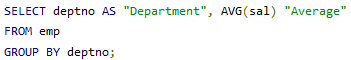
\includegraphics[]{res/themekorb_2/group_by.png}
\end{figure}

\subsubsection{HAVING}
\begin{itemize}
    \item Wird verwendet, wenn man das Ergebnis einer Gruppenfunktion als Bedingung haben möchte
    \begin{itemize}
        \item z.B. Durchschnittsgehalt aller Jobs, die ein durchschnittliches Gehalt $>$ 1500 haben:
    \end{itemize}
\end{itemize}
\begin{figure}[ht!]
    \centering 
    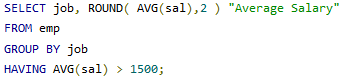
\includegraphics[]{res/themekorb_2/having.png}
\end{figure}

\subsection{Wichtige Funktionen}

\subsubsection{Case / Character}
\begin{itemize}
    \item LOWER / UPPER
    \item INITCAP $\implies$ Erster Buchstabe wird groß geschrieben!
    \item SUBSTR(string, start, length)
    \begin{itemize}
        \item Substring ab \textit{start} mit Länge von \textit{length}
    \end{itemize}
    \item LENGTH $\implies$ Länge des Strings
    \item LPAD / RPAD(column, length, 'ValueUsedForPadding')
    \item TRIM(string) $\implies$ Löscht Whitespaces an beiden Enden
    \begin{itemize}
        \item TRIM(string1, string2) $\implies$ Trimmt string2 von string1 (am Anfang und am Ende)
    \end{itemize}
    \item REPLACE(input, toBeReplaced, replaceWith) $\implies$ Ersetzt in Input den 2. String mit dem 3.
\end{itemize}

\subsubsection{Number}
\begin{itemize}
    \item ROUND(number, decimalPlaces) $\implies$ Rundet \textit{number} auf \textit{decimalPlaces} Nachkommastellen
    \item TRUNC(number, decimalPlaces) $\implies$ Schneidet \textit{number} nach \textit{decimalPlaces} Stellen ab
    \item MOD(number1, number2) $\implies$ number1 \% number2
\end{itemize}

\subsubsection{Date}
\begin{itemize}
    \item MONTHS\_BETWEEN(date1, date2) $\implies$ Anzahl der Monate dazwischen
    \item ADD\_MONTHS(date, numberOfMonths) $\implies$ Fügt \textit{numberOfMonths} Monate zu \textit{date} hinzu
    \item NEXT\_DAY(date, 'Day') $\implies$ Gibt den nächsten Wochentag \textit{nach} diesem Datum mit dem gewählten Namen zurück
    \item ROUND(date,  ['MONTH' | 'YEAR'])
    \begin{itemize}
        \item Rundet Auf das nächste / vorherige Jahr / Monat auf / ab
    \end{itemize}
    \item TRUNC(date, ['MONTH' | 'YEAR'])
    \begin{itemize}
        \item Setzt das Datum auf den 1. des Monats / Jahres
    \end{itemize}
\end{itemize}

\subsubsection{Conversion}
\begin{itemize}
    \item TO\_CHAR(columnWithDate | columnWithNumber, 'Format')
    \item TO\_NUMBER(input, 'Format')
    \begin{itemize}
        \item String zu Zahl parsen
    \end{itemize}
    \item TO\_DATE()
    \begin{itemize}
        \item String zu Datum parsen
    \end{itemize}
\end{itemize}
\begin{figure}[H]
    \centering 
    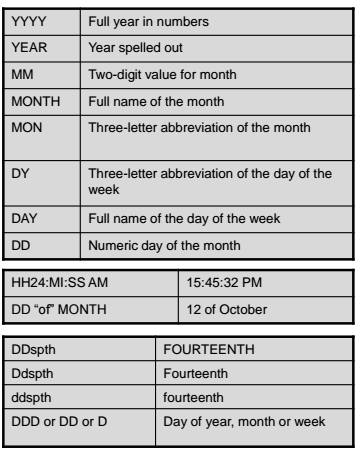
\includegraphics[]{res/themekorb_2/format.png}
\end{figure}
\subsubsection{Multi row}
\begin{itemize}
    \item MAX, MIN
    \item COUNT
    \item AVG
    \item SUM
    \item (STDDEV, VARIANCE)
\end{itemize}

\subsection{Joins}
\begin{itemize}
    \item Entweder mit ON oder mit USING
    \begin{itemize}
        \item INNER JOIN DEPT D ON EMP.DEPTNO = D.DEPTNO; $\implies$ Beide Spalten werden ausgegeben!
        \item INNER JOIN DEPT D USING(DEPTNO); $\implies$ Spalte muss in beiden Tables gleich heißen, wird nur 1x ausgegeben!
    \end{itemize}
\end{itemize}

\subsubsection{INNER JOIN}
\begin{itemize}
    \item Inkludiert nur Zeilen, die beiden Tables gleich sind!
\end{itemize}
\begin{figure}[H]
    \centering
    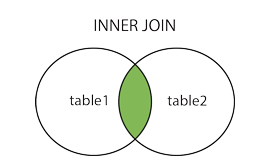
\includegraphics{res/themekorb_2/joins_inner_join.png} 
\end{figure}

\subsubsection{RIGHT OUTER JOIN}
\begin{itemize}
    \item Inkludiert alle Zeilen der rechten Tabelle (= die Tabelle, auf die gejoint wird) und Werte, die in beiden Tabellen gleich sind
    \begin{figure}[H]
        \centering
        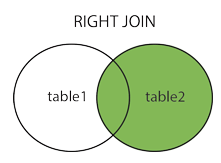
\includegraphics{res/themekorb_2/joins_right_outer_join.png} 
    \end{figure}
    \begin{itemize}
        \item Beispiel: Gib jene Abteilungen aus, die keine Mitarbeiter haben:
        \begin{figure}[H]
            \centering 
            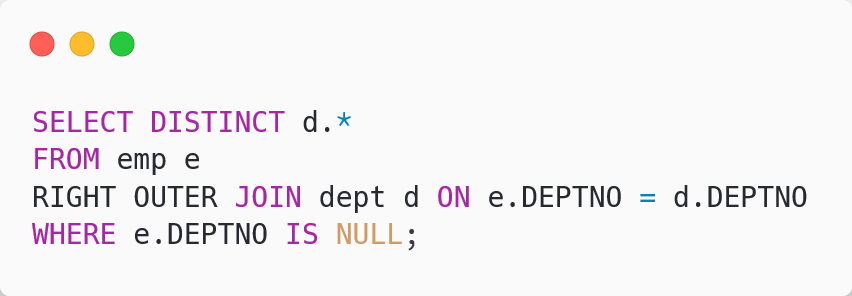
\includegraphics[scale=.45]{res/themekorb_2/joins_right_outer_join_example.png}
        \end{figure}
    \end{itemize}
\end{itemize}

\subsubsection{LEFT OUTER JOIN}
\begin{itemize}
    \item Inkludiert alle Zeilen der linken Tabelle (= die Tabelle, von der weg gejoint wird) und Werte, die in beiden Tabellen gleich sind
    \begin{figure}[H]
        \centering
        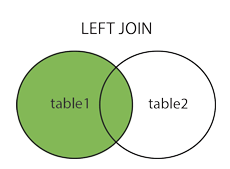
\includegraphics{res/themekorb_2/joins_left_outer_join.png} 
    \end{figure}
    \begin{itemize}
        \item Beispiel: Gib jene Abteilungen aus, die keine Mitarbeiter haben:
        \begin{figure}[H]
            \centering 
            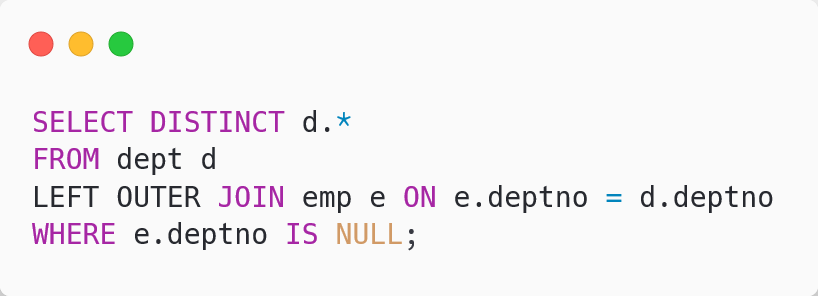
\includegraphics[scale=.45]{res/themekorb_2/joins_left_outer_join_example.png}
        \end{figure}
    \end{itemize}
\end{itemize}

\subsubsection{FULL OUTER JOIN}
\begin{itemize}
    \item Inkludiert alle Zeilen der linken Tabelle (= die Tabelle, von der weg gejoint wird) und alle Werte aus der rechten Tabelle
    \begin{figure}[H]
        \centering
        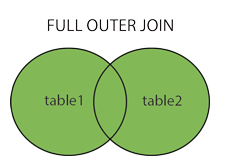
\includegraphics{res/themekorb_2/joins_full_outer_join.png} 
    \end{figure}
    \begin{itemize}
        \item Beispiel: Gib alle Mitarbeiter und Abteilungen aus
        \begin{figure}[H]
            \centering 
            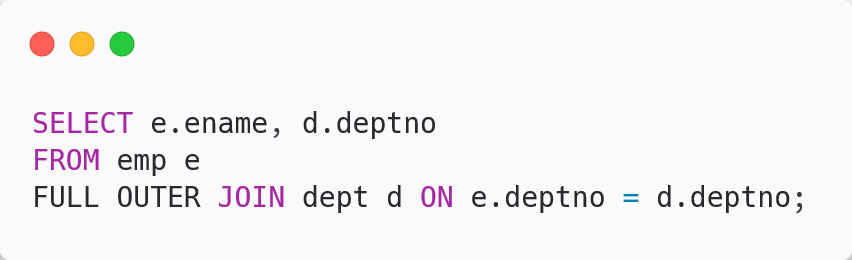
\includegraphics[scale=.45]{res/themekorb_2/joins_full_outer_join_example.png}
        \end{figure}
    \end{itemize}
\end{itemize}

\subsubsection{CROSS JOIN}
\begin{itemize}
    \item Gibt jede Zeile in einer Tabelle mit jeder Zeile aus einer anderen aus
    \item Problem: Auch jede Zeile mit sich selbst!
    \begin{figure}[H]
        \centering
        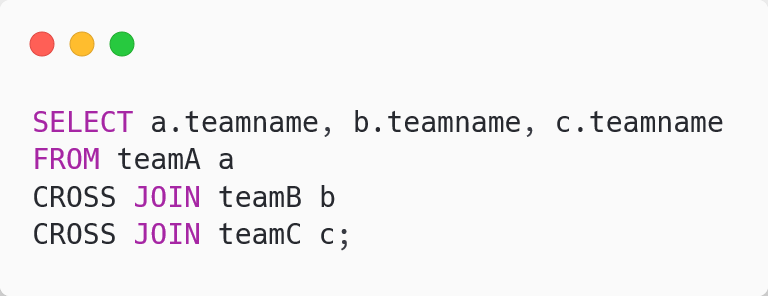
\includegraphics[scale=.4]{res/themekorb_2/cross_join.png} 
    \end{figure}
\end{itemize}

\subsubsection{SELF JOIN}
\begin{itemize}
    \item Es wird nochmal auf den gleichen Table gejoint (z.B. um den Vorgesetzten zu bestimmen)
\end{itemize}

\subsubsection{NATURAL JOIN}
\begin{itemize}
    \item Spalten, die beide Tabellen beinhalten werden nur 1x zurückgegeben!
    \item "Automatischer Inner Join" $\implies$ Es werden nur Spalten zurückgegeben, die den gleichen Wert haben (kein NULL!)
    \item Es wird AUF ALLE GLEICH BENANNTEN SPALTEN IN BEIDEN TABELLEN gejoint!
    \begin{itemize}
        \item Wenn eine neue Spalte hinzugefügt wird, welche zufällig so wie eine existierende heißt, werden nur Werte zurückgegeben, bei denen diese Spalten übereinstimmen!
    \end{itemize}
    \begin{figure}[H]
        \centering
        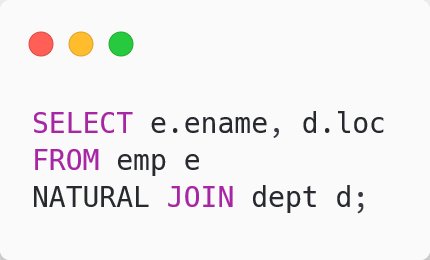
\includegraphics[scale=.4]{res/themekorb_2/natural_join.png} 
    \end{figure}
\end{itemize}

\subsubsection{EQUI / NON-EQUI Joins}
\begin{itemize}
    \item EQUI $\implies$ =
    \item NON-EQUI $\implies$ Alles andere (Größer / Kleiner, Between and\dots)
\end{itemize}

\subsection{Subselects}
\begin{itemize}
    \item Können in der WHERE, HAVING und FROM Klausel vorkommen
    \item Kann kein ORDER BY beinhalten
    \item Können eine (Single Row) oder mehrere (Multi-Row) Zeilen zurückliefern
    \begin{itemize}
        \item Single Row $\implies$ =, $<$, $>$, \dots
    \end{itemize}
    \item Wenn mehrere Werte aus dem Subselect zurückgegeben werden $\implies$ IN muss verwendet werden:
    \begin{figure}[H]
        \centering
        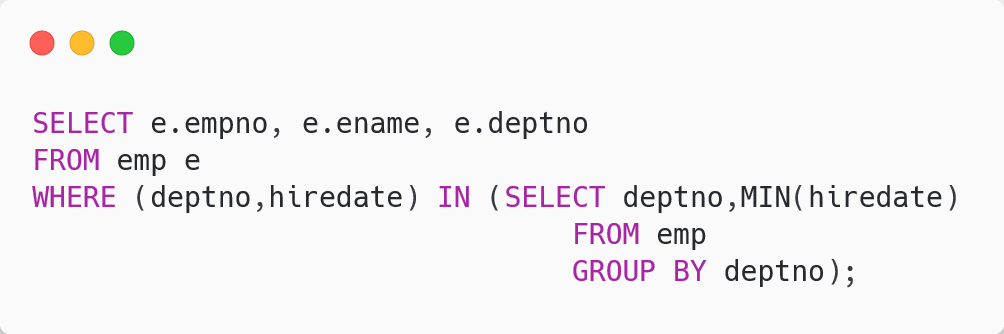
\includegraphics[scale=.4]{res/themekorb_2/subselect_multiple.png} 
    \end{figure}
\end{itemize}

\subsubsection{Multiple-Row Subselects}
\begin{itemize}
    \item Es müssen spezielle Operatoren verwendet werden:
    \begin{itemize}
        \item IN $\implies$ Es werden nur Zeilen zurückgegeben, dessen Wert in der Ergebnisliste des Subselects enthalten ist.
        \item ANY/SOME $\implies$ Ein Wert muss =, $<$, $>$ als irgendein Wert in der Ergebnisliste sein
        \item ALL $\implies$ Ein Wert muss =, $<$, $>$ als alle Werte in der Ergebnisliste sein
    \end{itemize}
    \item Correlation $\implies$ Es werden Werte von "Außen" in einer Subquery verwendet
\end{itemize}

\subsection{Andere, wichtige Keywords}
\subsubsection{UNION}
\begin{itemize}
    \item Der Output von 2 SQL-Statements kann verbunden werden
    \item \textbf{UNION ALL} $\implies$ Macht das gleiche, doppelte Werte werden allerdings angezeigt!
    \item Wichtig: Anzahl der Spalte + Datentypen müssen gleich sein, doppelte Werte werden ignoriert!
    \begin{figure}[H]
        \centering
        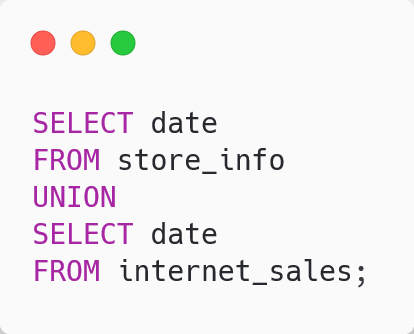
\includegraphics[scale=.4]{res/themekorb_2/union.png} 
    \end{figure}
\end{itemize}

\subsubsection{INTERSECT}
\begin{itemize}
    \item Gibt nur Werte aus, die in beiden Statements vorhanden sind!
    \begin{figure}[H]
        \centering
        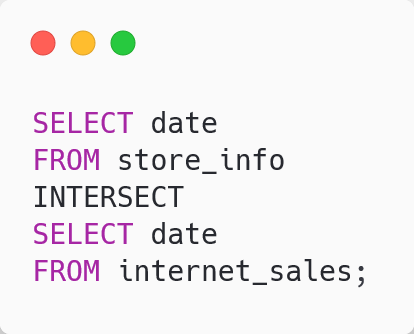
\includegraphics[scale=.4]{res/themekorb_2/intersect.png} 
    \end{figure}
\end{itemize}

\subsubsection{MINUS}
\begin{itemize}
    \item Gibt nur Werte aus, die in dem ersten Statement, nicht aber in dem 2. vorkommen!
    \begin{figure}[H]
        \centering
        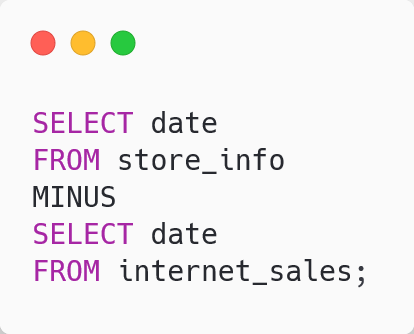
\includegraphics[scale=.4]{res/themekorb_2/minus.png} 
    \end{figure}
\end{itemize}

\subsection{Indizes}
\begin{itemize}
    \item Kann auf eine / mehrere (Composite Index) Spalten gleichzeitig angelegt werden
    \item Enthält den Wert + die zugehörige Spalte
    \item Muss bei jedem Insert / Delete / Update neu erstellt werden
\end{itemize}

\subsubsection{Wann?}
\begin{itemize}
    \item Es werden aus einem großen Table nur wenige Ergebnisse erwartet
    \item Die Spalte enthält häufig NULL Werte
\end{itemize}

\subsubsection{Wann nicht?}
\begin{itemize}
    \item Wenn die Tabelle oft bearbeitet / selten verwendet wird
    \item Wenn häufig mehr als 2-4\% der Tabelle ausgegeben werden
\end{itemize}

\subsubsection{Function based}
\begin{itemize}
    \item Die Werte im Index werden durch Funktionen berechnet:
    \begin{figure}[H]
        \centering
        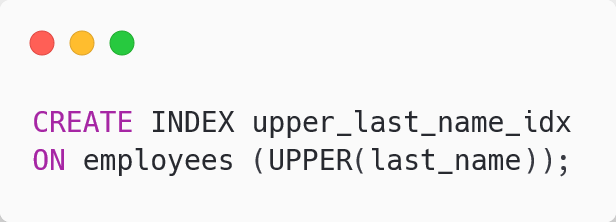
\includegraphics[scale=.4]{res/themekorb_2/function_based.png} 
    \end{figure}
    \item Es können auch selbst geschriebene Funktionen verwendet werden, diese müssen allerdings als "deterministic" markiert werden
\end{itemize}

\subsubsection{Erstellen \& Löschen}
\begin{itemize}
    \item Erstellen
    \begin{figure}[H]
        \centering
        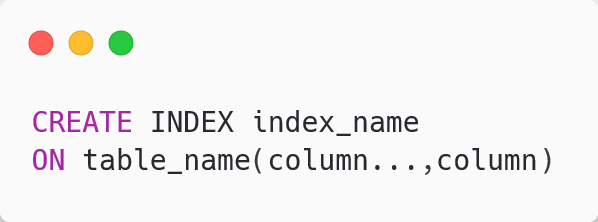
\includegraphics[scale=.4]{res/themekorb_2/create_index.png} 
    \end{figure}
    \item Löschen
    \begin{figure}[H]
        \centering
        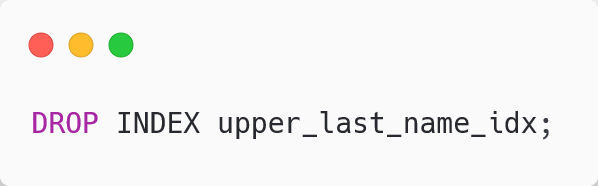
\includegraphics[scale=.4]{res/themekorb_2/drop_index.png} 
    \end{figure}
\end{itemize}

\subsection{Hierarchisches SQL}
\begin{itemize}
    \item Parent $\implies$ Wert über einer Node
    \item Child $\implies$ Wert unter einer Node
    \item Sibling $\implies$ Wert auf der gleichen Höhe
    \item Leaf $\implies$ Node ohne Child 
\end{itemize}

\subsubsection{Abfragen}
\begin{itemize}
    \item Pseudospalten
    \begin{itemize}
        \item LEVEL $\implies$ Level ab Root (hat Level 1)
        \item CONNECT\_BY\_ISCYCLE $\implies$ Gibt 1 zurück, wenn das Element Grund für einen Loop ist (letzter in der Hierarchie, bevor es von vorne los geht!)
        \item CONNECT\_BY\_ISLEAF $\implies$ Gibt 1 zurück, wenn das Element ein Leaf ist
    \end{itemize}
    \item Funktionen
    \begin{itemize}
        \item SYS\_CONNECT\_PATH(column, char) $\implies$ Pfad des Elements von der Root Node weg, getrennt durch \textit{char}
    \end{itemize}
    \item Operatoren
    \begin{itemize}
        \item SYS\_CONNECT\_BY\_ROOT $\impliedby$ Gibt den Wert der Spalte der Root Node zurück
        \item PRIOR $\impliedby$ Um Parent Nodes zu verbinden
    \end{itemize}
    \item Clauses
    \begin{itemize}
        \item START WITH \textit{condition} $\implies$ Auswahl der Root-Zeile
        \item CONNECT BY \dots PRIOR $\implies$ Gibt Verbindung zwischen Parent und Child an (mit PRIOR kann auf den Parent zugegriffen werden)
        \item ORDER SIBLINGS BY $\implies$ Sortiert die Siblings des Parents nach einer Spalte
    \end{itemize}
    \begin{figure}[H]
        \centering
        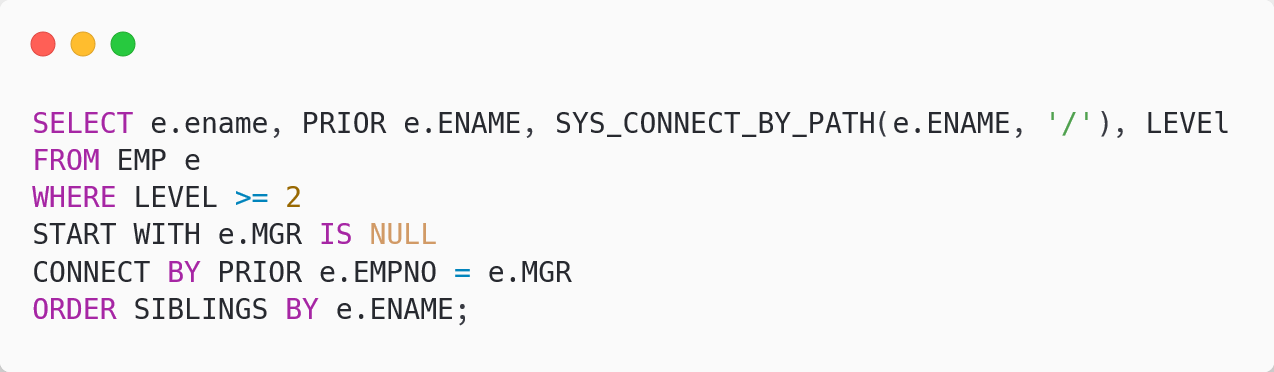
\includegraphics[scale=.3]{res/themekorb_2/hierarchical.png} 
    \end{figure}
\end{itemize}